%very helpful: https://latexdraw.com/plot-vector-field-in-latex-tikz/
\documentclass{standalone}
\usepackage{tikz}
\usepackage{pgfplots}
\pgfplotsset{compat = newest}
\usepgfplotslibrary{colormaps}

\begin{document}
	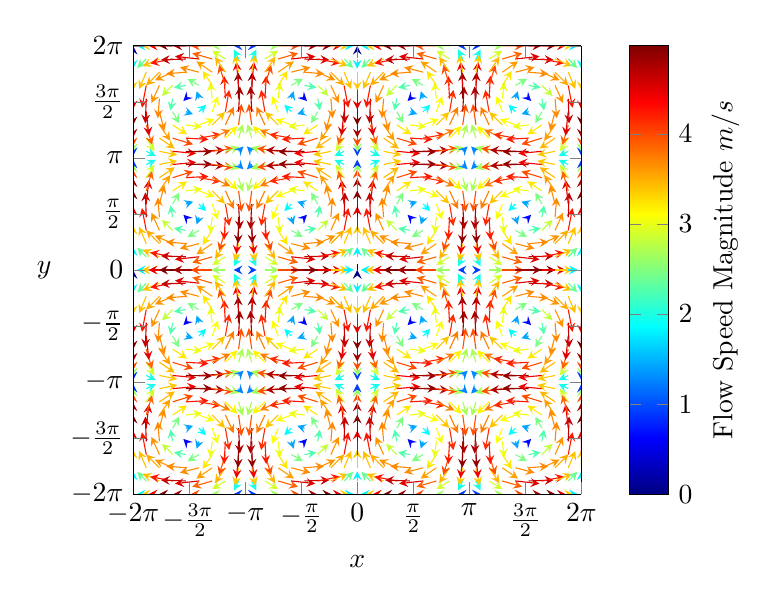
\begin{tikzpicture}
	\begin{axis}[
	domain=-2*pi:2*pi,
	xmin=-2*pi, xmax=2*pi,
	ymin=-2*pi, ymax=2*pi,
	zmin=0, zmax=1,
	axis equal image,
	view={0}{90},
	xtick = {-6.28318, -4.712389, ..., 4.712389, 6.28318},
	xticklabels={$-2\pi$, $-\frac{3\pi}{2}$, $-\pi$, $-\frac{\pi}{2}$, 0, $\frac{\pi}{2}$, $\pi$, $\frac{3\pi}{2}$, $2\pi$},
	ytick = {-6.28318, -4.712389, ..., 4.712389, 6.28318},
	yticklabels={$-2\pi$, $-\frac{3\pi}{2}$, $-\pi$, $-\frac{\pi}{2}$, 0, $\frac{\pi}{2}$, $\pi$, $\frac{3\pi}{2}$, $2\pi$},
	ylabel style={rotate=-90},
	xlabel={$x$},
	ylabel={$y$},
	colormap/jet,
	colorbar,
	colorbar style = {
		ylabel = {Flow Speed Magnitude $m/s$}}
	]
	\addplot3[
	point meta={sqrt((5*cos(deg(1*(x+(pi/(1*2)))))*sin(deg(1*(y+(pi/(1*2)))))*sin(deg(1*(0+(pi/(1*2))))))^2
		+(-5*sin(deg(1*(x+(pi/(1*2)))))*cos(deg(1*(y+(pi/(1*2)))))*sin(deg(1*(0+(pi/(1*2))))))^2)},
	quiver={
		u={5*cos(deg(1*(x+(pi/(1*2)))))*sin(deg(1*(y+(pi/(1*2)))))*sin(deg(1*(0+(pi/(1*2)))))},
		v={-5*sin(deg(1*(x+(pi/(1*2)))))*cos(deg(1*(y+(pi/(1*2)))))*sin(deg(1*(0+(pi/(1*2)))))},
		scale arrows = 0.15}, samples=35, quiver/colored={mapped color},-stealth
	]{0};
	\end{axis}
	\end{tikzpicture}
\end{document}